\documentclass{article}

\usepackage[
backend=biber,
style=numeric,
sorting=ynt
]{biblatex}
\addbibresource{refs.bib}

\usepackage{parskip}
\usepackage{amsmath}
\usepackage{amssymb}
\usepackage{mathtools}
\usepackage{needspace}
\usepackage{etoolbox}
\usepackage{listofitems}
\usepackage{xstring}
\usepackage{graphicx} % Required for inserting images
\usepackage{tikz}
\usetikzlibrary{patterns}
\usetikzlibrary{external}

\newtheorem{theorem}{Theorem}
\newtheorem{definition}{Definition}
\newtheorem{lemma}{Lemma}

\preto{\lemma}{\needspace{4cm}}
\preto{\section}{\needspace{5cm}}
\preto{\subsection}{\needspace{3cm}}

\title{Heart of the Four Color Theorem}
\author{Timothy van der Valk}
\date{November 2024 - January 2025}

\newcommand{\digitToNum}[1]{\the\numexpr#1\relax}
\newcommand{\scheme}[2]{
    \readlist*\mylist{#2}
     \tikz[baseline]{ 
        \foreach \x [count=\i] in {#1} {
            \coordinate (\i) at (0.3*\i, 0.225); \node[text height=0mm] at (0.3*\i,0) {$\x$};
        } 
        \foreachitem \z \in \mylist {
            \StrChar{\z}{1}[\left]
            \StrChar{\z}{2}[\right]
            \StrChar{\z}{3}[\color]
            \path (\left) edge[bend left=45] node[above, yshift=-2]{\small$\color$} (\right);
        }
    }
} 

\begin{document}

\maketitle

A new proof of the four-color theorem has been given by Thomas et al \cite{thomas} in 1995 as a response to the Appel and Haken proof from 1976. Both proofs of the four-color theorem depend on three smaller theorems and a set of configurations that together contradict the existence of a minimal counterexample. The difference is that the new proof has a set of 633 configurations compared to 1476 members of the old one.

Much of the difficulty from reading the proof of the four-color theorem comes from the confusing language of dated papers and incomplete or hasty steps in proofs. This document elaborates on such details left out by the original papers and papers and tries to put a logical order to it all.


\tableofcontents

\pagebreak
\section{Introduction}

The four-color theorem is proven by disproving the existence of minimal counterexamples. Let us begin by defining such a minimal counterexample.
\begin{definition}
A graph $G$ is a minimal counterexample to the four-color theorem if $G$ is not four-colorable but any graph $H$ of lower weight $|V(H)|+|E(H)|$ is.
\end{definition}

All minimal counterexamples we mention will be those of the four-color theorem.
The three theorems to the four-color theorem are then as follows. We leave further definitions to Sections \ref{sec:birkhoff} and \ref{sec:config}.

\begin{theorem}
Minimal counterexamples are Birkhoff graphs.
\end{theorem}

\begin{theorem}
Minimal counterexamples do not contain configurations.
\end{theorem}

\begin{theorem}
Birkhoff graphs contain a configuration.
\end{theorem}

Clearly these three results contradict each other. Minimal counterexamples are proven to have no configurations, but subsequently through Birkhoff graphs, do in fact have configurations. This is a contradiction. As a consequence, there can not exist any minimal counterexamples and the four-color theorem is true. 

Theorem 1 is proven by hand in Section \ref{sec:birkhoff}. Theorem 2 and 3 are explained in Section \ref{sec:config} but require a computer to verify all cases. Birkhoff graphs are also called "internally 6-connected triangulations" in literature, but we will use the former for readability.

\section{Birkhoff Reducibility}
\label{sec:birkhoff}

Before 1913, the only known reductions of maps we're the reductions to triangulations and the reduction of multiply-connected regions to fewer regions (holed regions). In 1913, Birkhoff \cite{birkhoff} proved a new reduction result for \textit{rings} that seperate two parts of a map. This result spurred new developments in the reduction of graphs that opened the path towards reducible configurations and finally the proof of Appel and Haken in 1976.

We will use the term \textit{map} to refer to a map of connected \textit{regions} that we wish to four-color. From such a map we can construct a \textit{planar graph} where each region represents a vertex. We will be working with graphs in all our proofs, but might sometimes mention maps for intuition. We denote by $|G|$ the number of vertices in the graph $G$.

Let us begin by defining a ring of a graph.

\begin{definition}
    A ring of $n$ vertices $R_n$ in a graph $G$ is an induced cycle of $G$ that encloses at least one vertex.
\end{definition}

The key property of rings is that they seperate the full graph $G$ in three parts $M_1$, $R$ and $M_2$. That is, $G$ is of the form $G = M_1 + R + M_2$. The notation $A + B$ indicates a \textbf{direct} connection between the subgraphs $A$ and $B$. Since the ring seperates $M_1$ and $M_2$, they are not directly connected together.

\begin{figure}[!ht]
    \centering
        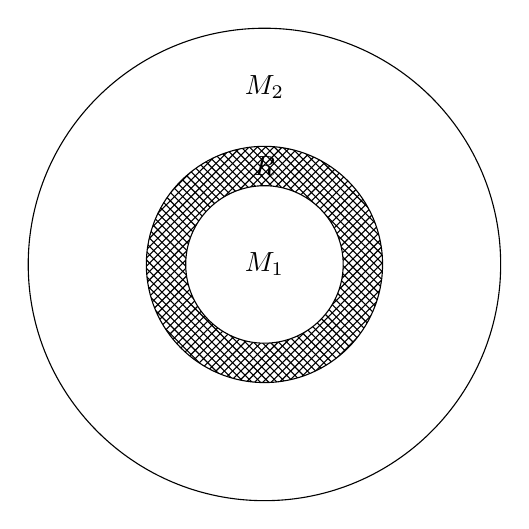
\begin{tikzpicture}
        \draw[fill=white] (0,0) circle (3cm);
        \draw[fill opacity=0.4, pattern=crosshatch] (0,0) circle (1.5cm);
        \draw[fill=white] (0,0) circle (1cm);
        \node at (0, 1.25) {$R$};
        \node at (0, 2.25) {$M_2$};
        \node at (0, 0) {$M_1$};
    \end{tikzpicture}
    \caption{The graph $G = M_1 + R + M_2$.}
\end{figure}

To reduce a ring like this, we may try to color $M_1+R$ and $M_2+R$ individually such that the colors on $R$ agree. Then we can combine both colorings together to form a coloring of the full graph $G$. This is the key idea of Birkhoff reducibility.

However, we do not know if such a common coloring of $M_1+R$ and $M_2+R$ always exists. Birkhoff's paper concerned itself with the conditions under which this, or a weaker result, is possible.

\subsection{Kempe Chains and Ring Schemes}

To make our coloring proofs easier, we need some definitions and notation to rewrite one coloring to another more easily. We will begin by defining chains of alternating colors connected to a vertex $v$.

\begin{definition}
    Given two colors $a,b$ and a coloring of a graph $G$. The $ab$-chain of a vertex $v \in G$ consists of all vertices colored $a,b$ that are connected to $v$ through other vertices colored $a,b$.
\end{definition}

Given a coloring of $M+R$. Consider the $ab$-chains of two vertices $v_1$ and $v_2$ on the ring $R$. If these chains are connected, then we may flip the colors in both $ab$-chains together to obtain a single new coloring. If these chains are not connected, then we may flip each $ab$-chain individually to obtain three new colorings ($\circ \bullet, \bullet \circ$ and $ \bullet \bullet$) instead.

Therefore, by using the concept of chains we can rewrite one coloring to another given knowledge of the chains that are present. To know which chains are present on a ring $R$, we also introduce the concept of a \textbf{ring scheme}.

\begin{definition}
    A ring scheme consists of the colors of a ring $R_n$ where two colors of the scheme are connected by a line if the corresponding vertices are connected by a chain. The colors in the chain are indicated above the line.
\end{definition}

For example, \scheme{a,b,a,b}{13c} indicates that the ring is colored $abab$ with a chain connecting $v_1$ and $v_3$.

\begin{figure}[!ht]
    \centering
    
    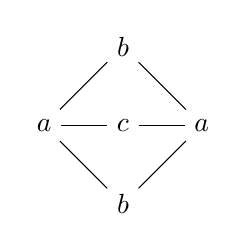
\begin{tikzpicture}
        % Define the nodes
        \node (v1) at (-1, 0) {$a$};
        \node (v2) at (0, 1) {$b$};
        \node (v3) at (1, 0) {$a$};
        \node (v4) at (0, -1) {$b$};
        \node (c) at (0, 0) {$c$};

        % Draw the edges
        \draw (v1) -- (v2) -- (v3) -- (v4) -- (v1);
        \draw (v1) -- (c) -- (v3);
    \end{tikzpicture}
    \caption{A graph that is colored $abab$ and has an $ac$-chain.}
\end{figure}

Now given the scheme \scheme{a,b,a,b}{13c}, we know certainly that there can not exist a $bd$-chain connecting $v_2$ and $v_4$ on the same side as the $ac$-chain. See the above graph, for example. Thus we can flip $v_2$ safely to obtain a new coloring $adab$. In such a case we write $\scheme{a,b,a,b}{13c} \cong \scheme{a,d,a,b}{13c}$. In addition, we write $abab \cong \scheme{a,b,a,b}{13d}$ to state that the coloring $abab$ has the specified ring scheme.

In general, if there is a chain connecting two vertices on the ring, then there can not exist a chain in complementary colors connecting two vertices seperated by that chain on the same ring.

\subsection{Ring Reducibility Numbers $\phi(n)$}

As we will prove in the next two sections, we can reduce the coloring of a graph containing the rings $R_4$ and $R_5$ as follows.

\begin{figure}[!ht]
    \centering
    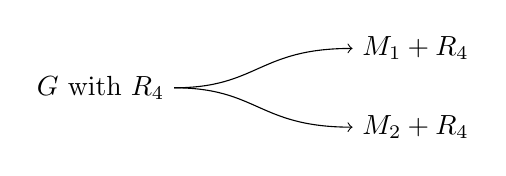
\begin{tikzpicture}
        \node (r4) at (-5, 0) {$G$ with $R_4$};
        \node (r4a) at (-1, 0.5) {$M_1+R_4$};
        \node (r4b) at (-1, -0.5) {$M_2+R_4$};
        \draw[->] (r4) .. controls +(2, 0) and (-3, 0.5) ..(r4a);
        \draw[->] (r4) .. controls +(2, 0) and (-3, -0.5) ..(r4b);
    \end{tikzpicture}
    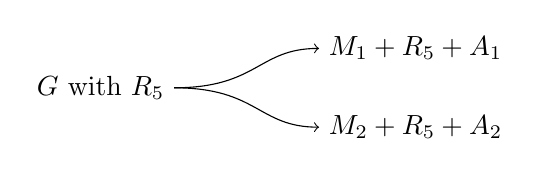
\begin{tikzpicture}
        \node (r4) at (-5, 0) {$G$ with $R_5$};
        \node (r4a) at (-1, 0.5) {$M_1+R_5+A_1$};
        \node (r4b) at (-1, -0.5) {$M_2+R_5+A_2$};
        \draw[->] (r4) .. controls +(2, 0) and (-3, 0.5) ..(r4a);
        \draw[->] (r4) .. controls +(2, 0) and (-3, -0.5) ..(r4b);
    \end{tikzpicture}
    \caption{The two key results of ring reducibility by Birkhoff. Rings of size 5 can only be reduced with auxiliary vertices $|A_1|=1$ and $|A_2| \leq 1$.}
\end{figure}

We have that rings of size 4 can be reduced exactly as we sought. However, for rings of size 5, at least one of the reduced graphs requires an auxiliary vertex. This is a slightly weaker result. In fact, the larger the ring size, the more auxiliary vertices will be required.

Birkhoff identified this as the generalization of ring reducibility and gave it a definition. 

\begin{definition}
    Let $\phi(n) = k$ where $k$ is the lowest integer such that all graphs $M_1+R_n+A_1$ and $M_2+R_n+A_2$ have a common ring coloring on $R_n$ for some $A_1$ and $A_2$ with $|A_1|=k$ and $|A_2|\leq k$ that are connected to all vertices of $R_n$.
\end{definition} 

We will be able to reduce graphs with rings of size $n$ to two \textbf{smaller}  graphs as long as $M_1$ and $M_2$ both contain more than $\phi(n)$ vertices. Otherwise, we would be reducing to a graph $|M+R_n+A| = |G|$, which is useless.

\subsection{Proof that $\phi(4)=0$}

We are now ready to prove that rings of size 4 are reducible without auxiliary regions ($k=0$). Let the ring colorings of $M_1+R_4$ be given by I, and the ring colorings of $M_2+R_4$ by II. 

Since we can reduce cycles of size greater than three to triangles, we can color two vertices on the ring $R_4$ the same. We can merge either $v_1$ and $v_3$, or $v_2$ and $v_4$. This results in colorings $a{*}a{*}$ and ${*}a{*}a$ where the $*$ are yet to be decided.

If the ring requires only two colors, then the only coloring we get is of the form $abab$. If the ring requires three colors, we get either $abac$ or $baca$ (up to permutation). Therefore we have two sets of choices for I and II.

\begin{equation*}
    abab, \quad\quad abac+baca
\end{equation*}

If I and II have the same type of coloring, we are done. Therefore, suppose that we have $\text{I}(abab)$  and $\text{II}(abac+baca)$. We will show that $abab$ can be rewritten to a coloring for II by branching on the existence of chains.

Suppose that there is an $ad$-chain connecting $v_1$ and $v_3$ in $\text{I}(abab)$. Then we have
\begin{equation*}
    \text{I}(abab) \cong \scheme{a,b,a,b}{13d}  \cong \text{II}(abac)
\end{equation*}

If there is no such chain, we must have a $bc$-chain connecting $v_2$ and $v_4$ such that 
\begin{equation*}
    \text{I}(abab) \cong \scheme{a,b,a,b}{24c} \cong \text{II}(baca)
\end{equation*}

In either case we get that $|\text{I} \cap \text{II}| > 0$, i.e there is a common ring coloring of $M_1+R_4$ and $M_2+R_4$. Hence $\phi(4) = 0$ since no auxiliary vertices we're used.

\subsection{Proof that $\phi(5)\leq1$}

To prove that $\phi(5)=1$, we first show that we can always find a common coloring of $M_1+R_5+A_1$ and $M_2+R_5+A_2$ if $|A_1|=1$ and $|A_2|\leq 1$ such that $\phi(5) \leq 1$. Then we give a counterexample such that $\phi(5)\neq 0$.

Let us consider the ring colorings I of the graph $M_1 + R_5 + A_1$. We have a single auxiliary vertex in $A_1$ that is connected to all vertices of the ring $R_5$. Since we can use only four colors, the ring has three colors with the last being used on $A_1$. Therefore we have \textbf{one of} the colorings

\begin{equation*}
    \vec{\underline{c}}abab = \begin{cases}
        cabab, \\
        acbab, \\
        abcab, \\
        abacb, \\
        ababc
    \end{cases}
\end{equation*}

The shorthand $\vec{c}abab$ indicates that $c$ can change position freely. We can only assume to have one of these colorings in I. The underlined vertex is called the \textbf{marked vertex}. This is the uniquely colored vertex in a three-coloring. Two three-colorings are called \textbf{adjacent} if the marked vertices are adjacent. 

Now for the ring colorings II of the graph $M_2+R_5+A_2$ we may consider $|A_2|=0$ and $1$. We have the colorings for $|A_2|=1$ as above. For $|A_2|=0$, we will be left with $M_2+R_5$. Again, cycles of size greater than three may be reduced by merging any two opposite vertices. This results in \textbf{all of} the following colorings

\begin{equation*}
    \vec{\underline{c}}abab, \quad\quad
    +\vec{a}{*}\vec{a}{*}{*} = \begin{cases}
        a{*}a{*}{*}+ \\
        {*}a{*}a{*}+ \\
        {*}{*}a{*}a+ \\
        a{*}{*}a{*}+ \\
        {*}a{*}{*}a
    \end{cases}
\end{equation*}

Here the shorthand $+\vec{a}{*}\vec{a}{*}{*}$ to indicates that the we have \textbf{all} valid colorings where $a$ can change position freely. The starred colors \textbf{depend} on the positions of $a$. Each coloring requires either three or four colors.

Now we can begin to show that there is a common ring coloring in I and II. We will do this by proving the following two lemmas.

\begin{lemma}
    \label{r5lem1}
    If I and II have two non-adjacent colorings, then they either have adjacent colorings or a common coloring.
\end{lemma}

\begin{lemma}
    \label{r5lem2}
    If I and II have two adjacent colorings, then they have a common coloring.
\end{lemma}

Together these two lemmas imply that regardless of whether the two colorings $\vec{\underline{c}}abab$ in I and II are adjacent or non-adjacent, there will be a common coloring. If the marked vertices are the same, we can simply permute colors to obtain a common coloring.

\vspace{1em}
\emph{Proof of Lemma \ref{r5lem1}}

Assume we have two non-adjacent colorings $\text{I}(ab\underline{c}ab)$ and $\text{II}(\underline{c}abab)$. If a $bc$-chain connects $v_3$ and $v_4$ in $\text{I}(ab\underline{c}ab)$, then we obtain

\begin{equation*}
    \text{I}(ab\underline{c}ab) \cong \scheme{a,b,c,a,b}{35} \cong \text{I}(abcdb)
\end{equation*}

Let us now consider the coloring $\text{II}({*}b{*}{*}b)$. We must certainly use three colors, so we have at least $\text{II}({*}bcdb)$ with three options for the last color.

\begin{equation*}
    \text{II}({*}bcdb) \cong \begin{cases}
        \text{II}(abcdb) \cong& \text{I}(abcdb), \\
        \text{II}(cbc\underline{d}b) \quad \text{adjacent to} \quad& \text{I}(ab\underline{c}ab), \\
        \text{II}(db\underline{c}db) \cong& \text{I}(ab\underline{c}db)
    \end{cases}
\end{equation*}

In all three cases, we either have a common coloring or an adjacent coloring in I and II. If a $bc$-chain did not exist, then we have an $ad$-chain between $v_1$ and $v_4$ such that 

\begin{equation*}
    \text{I}(ab\underline{c}ab) \cong \scheme{a,b,c,a,b}{14d} \cong \text{I}(a\underline{c}bab)\quad \text{adjacent to}\quad \text{II}(\underline{c}abab).
\end{equation*}

An equivalent argument holds for all other pairs of non-adjacent colorings. Therefore we have either an adjacent coloring or a common coloring in I and II regardless of the colorings in I and II.

\vspace{1em}
\emph{Proof of Lemma \ref{r5lem2}}

Assume we have $\text{I}(a\underline{c}bab)$ and $\text{II}(\underline{c}abab)$. If a $bc$-chain connects $v_2$ and $v_4$ in $\text{I}(b\underline{c}aba)$, then we obtain

\begin{equation*}
    \text{I}(b\underline{c}aba) \cong \scheme{b,c,a,b,a}{24} \cong \text{I}(bcdba)
\end{equation*}

Now consider the coloring $\text{II}(b{*}{*}b{*})$. We again have three cases for this coloring starting from $\text{II}(bcdb{*})$.

\begin{equation*}
    \text{II}(bcdb{*}) \cong \begin{cases}
        \text{II}(bcdba) \cong& \text{I}(bcdba), \\
        \text{II}(bc\underline{d}bc) \\
        \text{II}(b\underline{c}dbd) \cong& \text{I}(a\underline{c}bab)
    \end{cases}
\end{equation*}

Now in case we obtain the coloring $\text{II}(bc\underline{d}bc)$, we have essentially shifted two steps right from $\text{II}(\underline{c}abab)$. If we repeat the same argument with $\text{II}(bc\underline{d}bc)$ and $\text{I}(a\underline{c}bab)$, we will obtain $\text{I}(aba\underline{c}b)$. Hence by repetition we get the colorings

\begin{equation*}
    \stackrel{\text{start}}{\text{I}(a\underline{c}bab)} \rightarrow 
    \text{I}(aba\underline{c}b) \rightarrow 
    \text{I}(\underline{c}abab) \cong \text{II}(\underline{c}abab)
\end{equation*}

The same repetition argument holds for all other pairs of adjacent colorings in I and II too. Therefore, if there adjacent colorings in I and II, then we obtain a common coloring of I and II.

Since we have proven both Lemma's, we conclude that the ring of five regions is reducible with $\phi(5) \leq 1$.

\subsection{Proof that $\phi(5) \neq 0$}

To prove that $\phi(5) \neq 0$, we must give an example of two  of graphs $M_1+R_5$ and $M_2+R_5$ such that there is no common ring coloring.




\section{Configurations}
\label{sec:config}

\section{C/D Reducibility}
\label{sec:reduce}

\pagebreak
\printbibliography

\end{document}
